\documentclass{standalone}
\usepackage{picture,color}
\usepackage{graphicx}
\graphicspath{{./Fig_PFC_subfigs/}}
\setlength{\unitlength}{1in}
\renewcommand{\rmdefault}{phv} % Arial
\renewcommand{\sfdefault}{phv} % Arial

\begin{document}
\begin{picture}(6.85, 6.55)(0,-6.8)
% example frame 
\put(0.15, -1.4){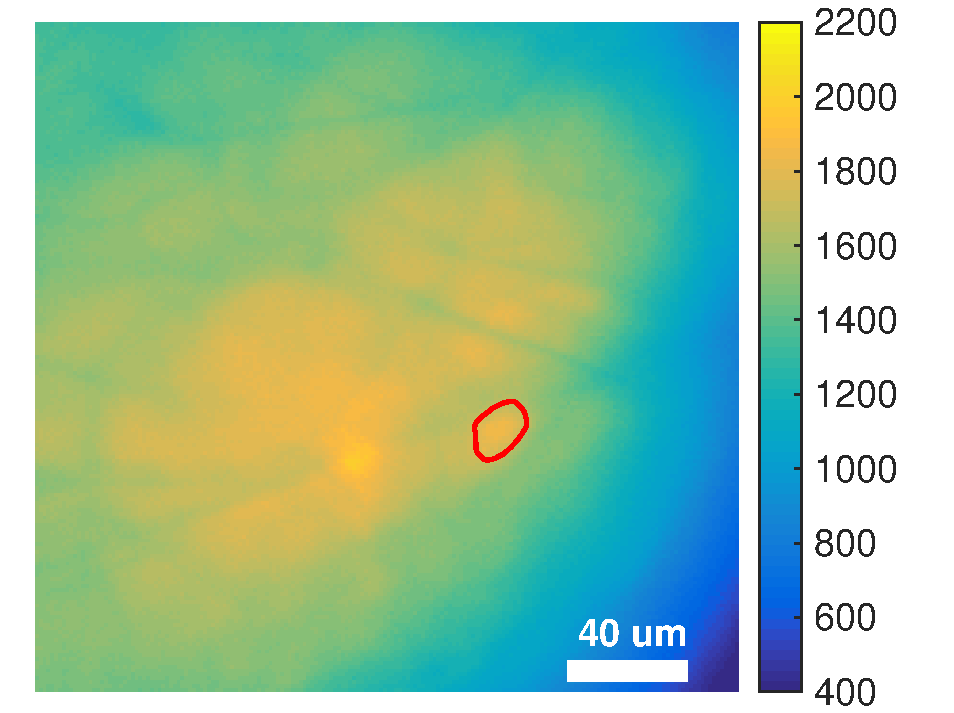
\includegraphics[height=1in]{Fig_PFC_subfigs/example_frame.pdf}}
\put(0.02, -0.45){\large\textbf{A}}
\put(.40, -0.4){\scriptsize Raw data}

\put(1.4,-0.95){\large\textbf{=}}
\put(1.50, -1.4){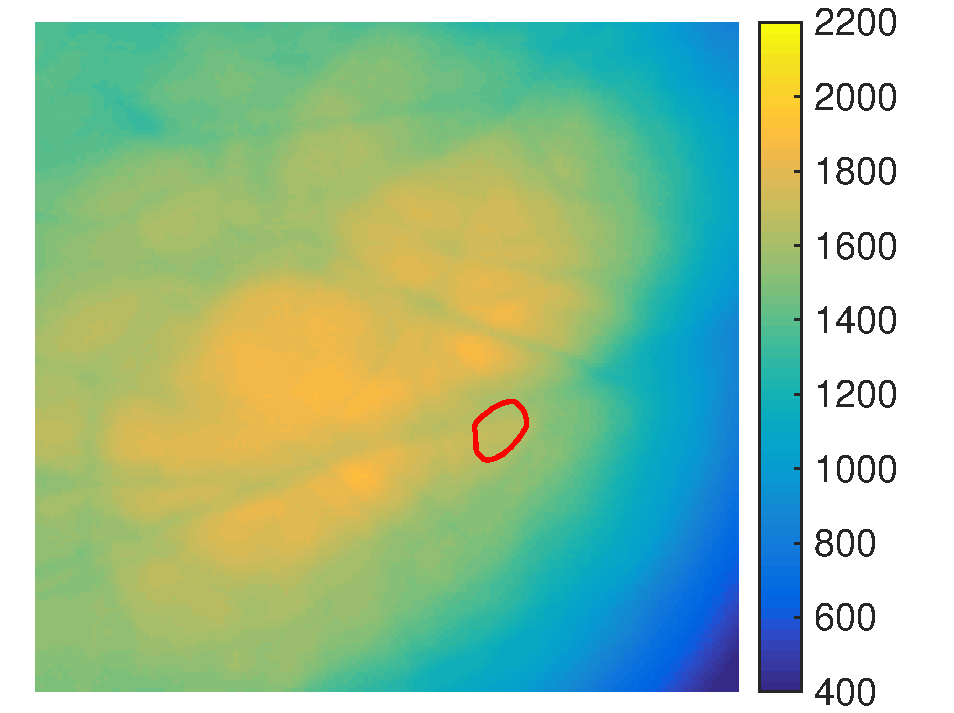
\includegraphics[height=1in]{Fig_PFC_subfigs/example_frame_bg_constant.pdf}}
\put(1.63, -0.4){\scriptsize Const. baseline}

\put(2.75,-0.95){\large\textbf{+}}
\put(2.85, -1.4){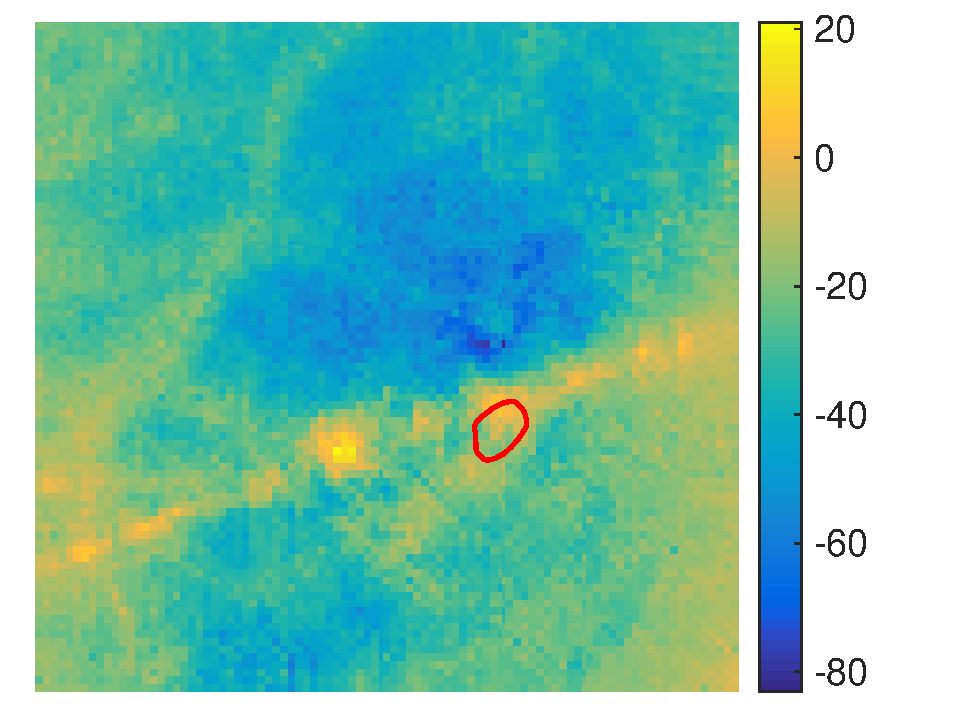
\includegraphics[height=1in]{Fig_PFC_subfigs/example_frame_bg_fluc.pdf}}
\put(2.94, -0.4){\scriptsize Fluc. background}

\put(4.1,-0.95){\large\textbf{+}}
\put(4.2, -1.4){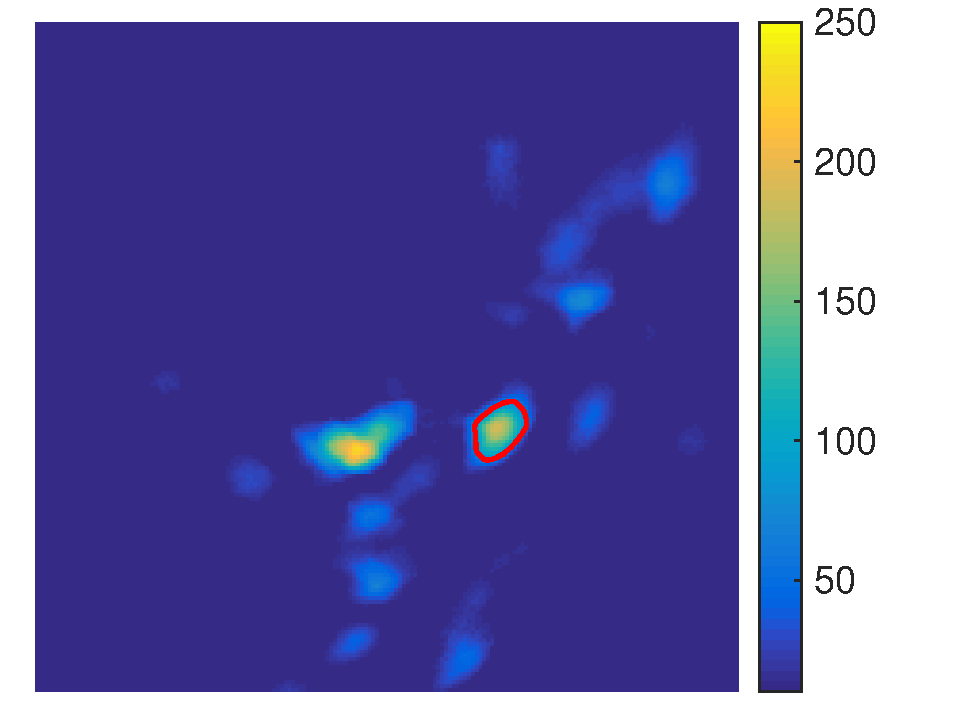
\includegraphics[height=1in]{Fig_PFC_subfigs/example_frame_ac.pdf}}
\put(4.37, -0.4){\scriptsize Neural signal}

\put(5.45,-0.95){\large\textbf{+}}
\put(5.55, -1.4){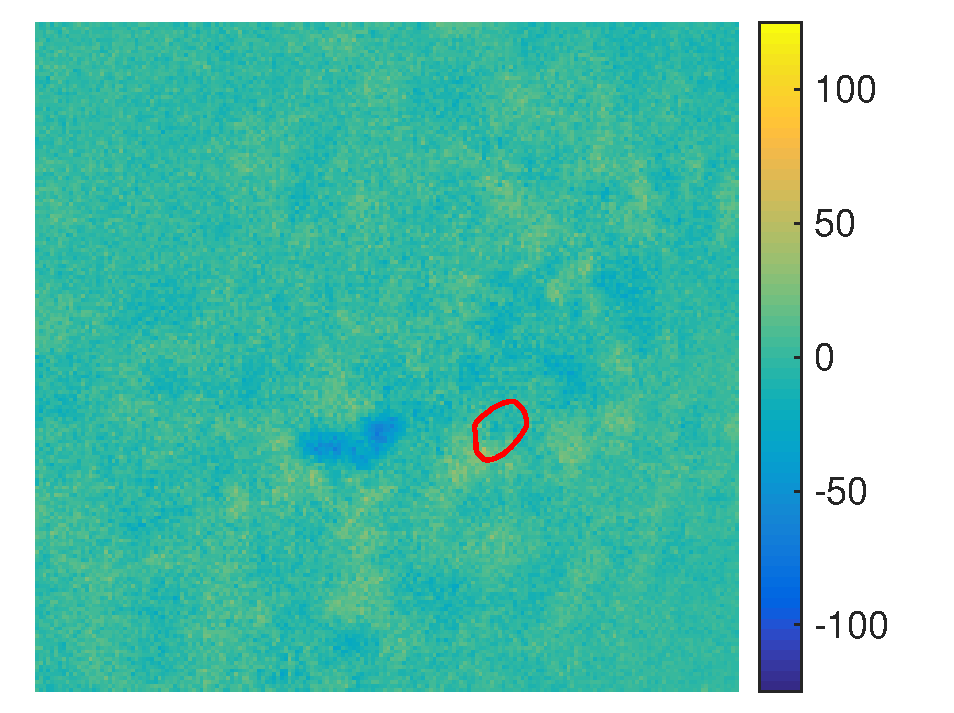
\includegraphics[height=1in]{Fig_PFC_subfigs/example_frame_res.pdf}}
\put(5.8, -0.4){\scriptsize Residual}

% % traces within an selected ROI 
\put(0.08, -3.0){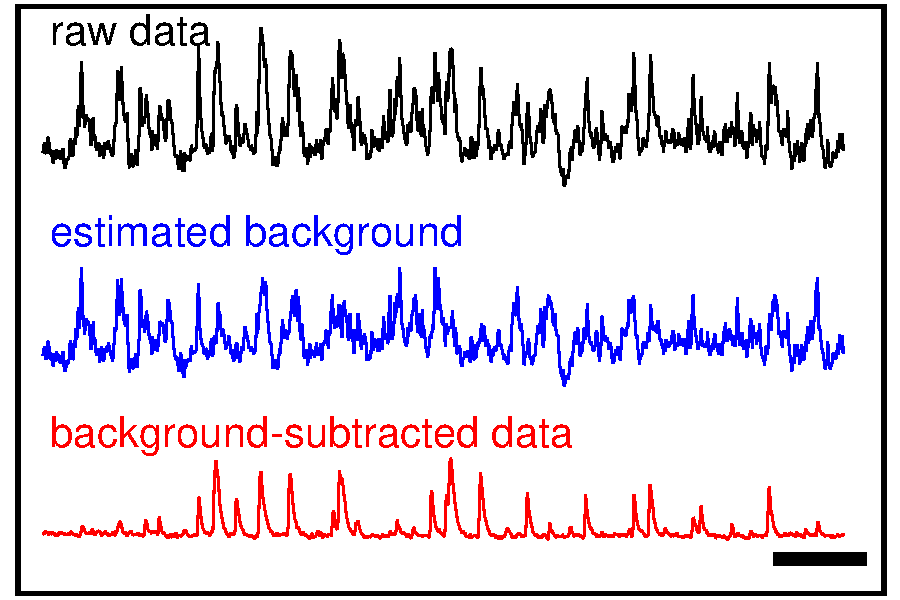
\includegraphics[height=1.43in]{Fig_PFC_subfigs/example_roi_traces.pdf}}
\put(0.02, -1.59){\large\textbf{B}}
\put(0.55, -1.53){\scriptsize Fluorescence traces within the ROI}

% contour plot  
\put(4.9, -4.785){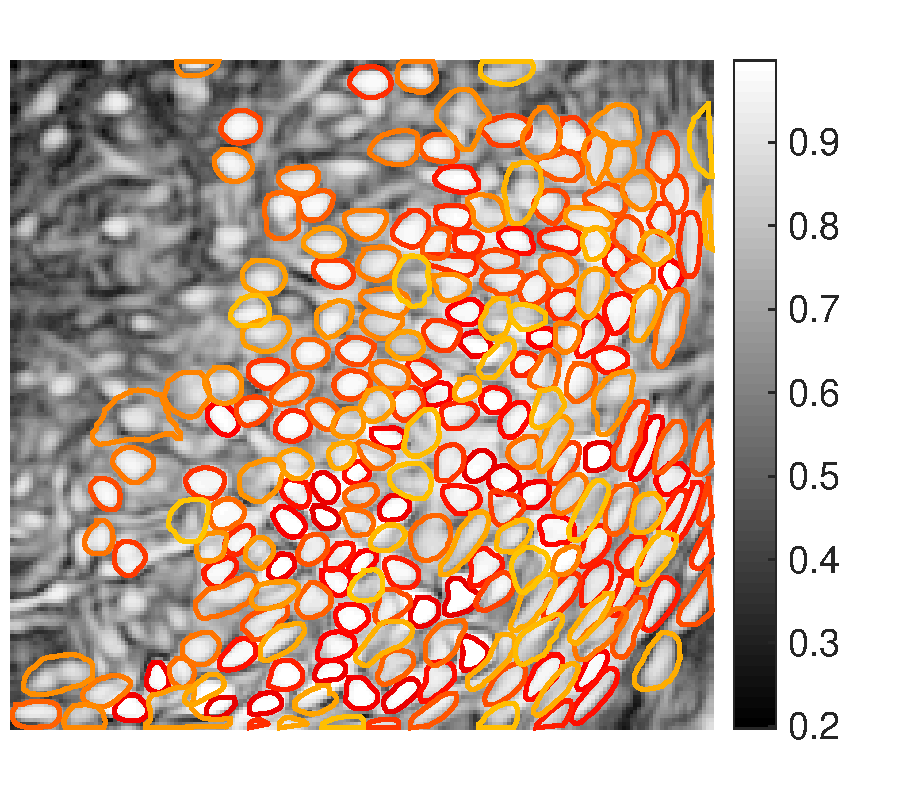
\includegraphics[height=1.58in]{Fig_PFC_subfigs/contours_ica.pdf}}
\put(4.9, -3.185){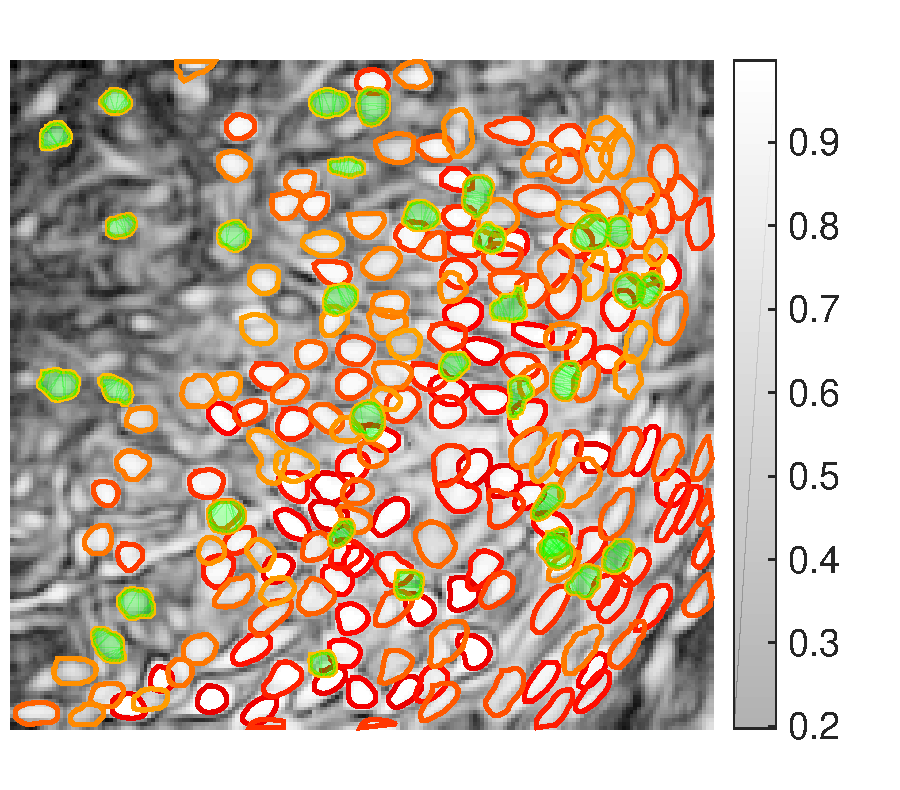
\includegraphics[height=1.58in]{Fig_PFC_subfigs/contours_cnmfe.pdf}}
\put(4.6, -1.59){\large\textbf{D}}
\put(5.5, -1.53){\scriptsize Contour plot}
\put(4.72, -1.59){\line(1,0){2.08}}
\put(6.8,-1.59){\line(0, -1){3.2}}
\put(4.72, -1.59){\line(0,-1){3.2}}
\put(4.72, -4.79){\line(1,0){2.08}}
\put(4.77, -2.7){\rotatebox{90}{CNMF-E}}
\put(4.77, -4.3){\rotatebox{90}{PCA/ICA}}


\put(0.18, -3.62){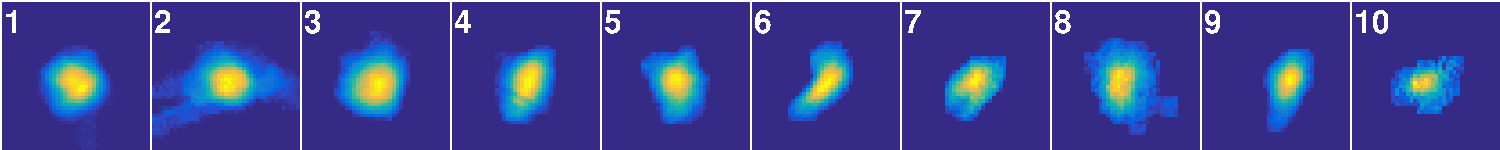
\includegraphics[height=0.3in]{Fig_PFC_subfigs/ica_missed_spatial.pdf}}
\put(0.02, -4.9){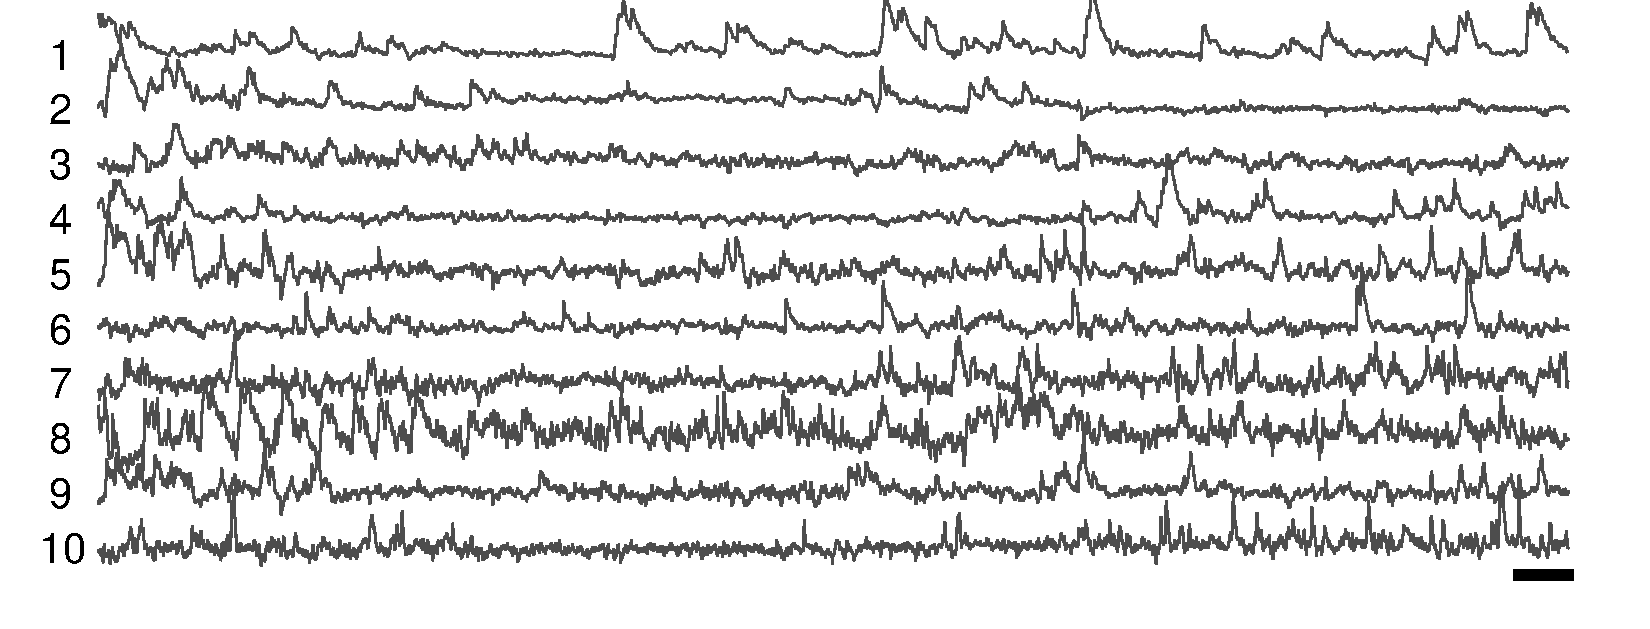
\includegraphics[height=1.2in]{Fig_PFC_subfigs/ica_missed_temporal.pdf}}
\put(0.02, -3.33){\large\textbf{E}}
\put(0.82, -3.28){\scriptsize Components detected by CNMF-E only}

\put(3.38, -5.05){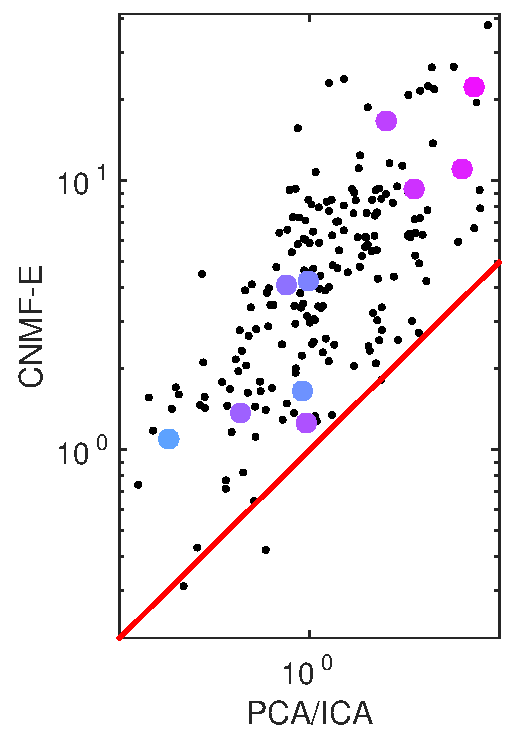
\includegraphics[height=1.73in]{Fig_PFC_subfigs/snr_pca_ica.pdf}}
\put(3.33, -3.33){\large\textbf{F}}
\put(3.98, -3.28){\scriptsize SNR}

% matched neurons 
\put(0.2, -6.6){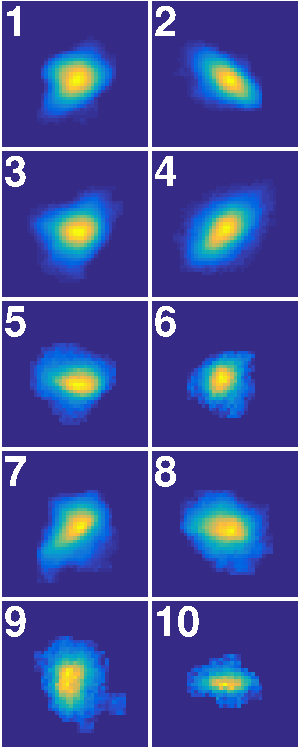
\includegraphics[height=1.5in]{Fig_PFC_subfigs/match_spatial_cnmfe.pdf}}
\put(0.85, -6.6){\includegraphics[height=1.5in]{Fig_PFC_subfigs/match_spatial_ICA.pdf}}
\put(0.02, -5.13){\large\textbf{G}}
\put(0.31, -5.08){\scriptsize CNMF-E}
\put(0.96, -5.08){\scriptsize PCA/ICA}


\put(4.05, -6.75){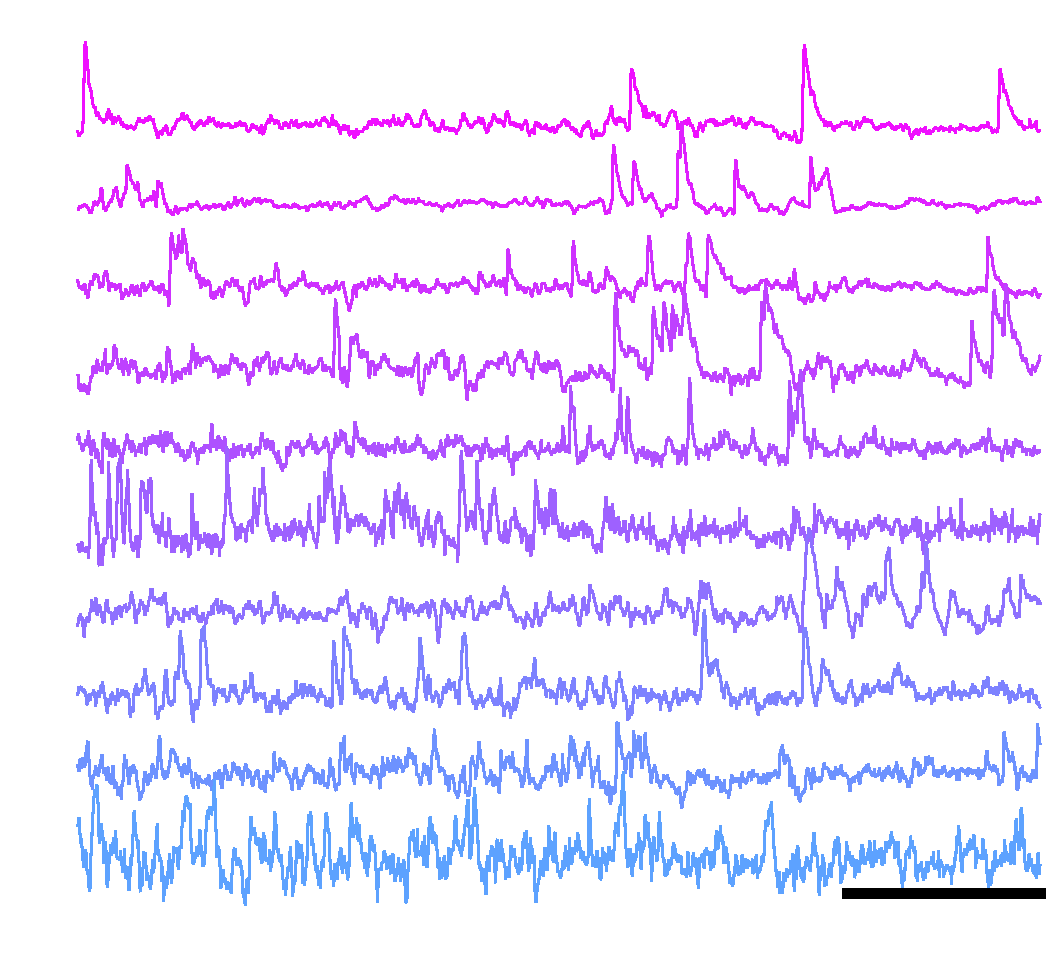
\includegraphics[height=1.65in]{Fig_PFC_subfigs/matched_temporal_ica.pdf}}
\put(1.55, -6.75){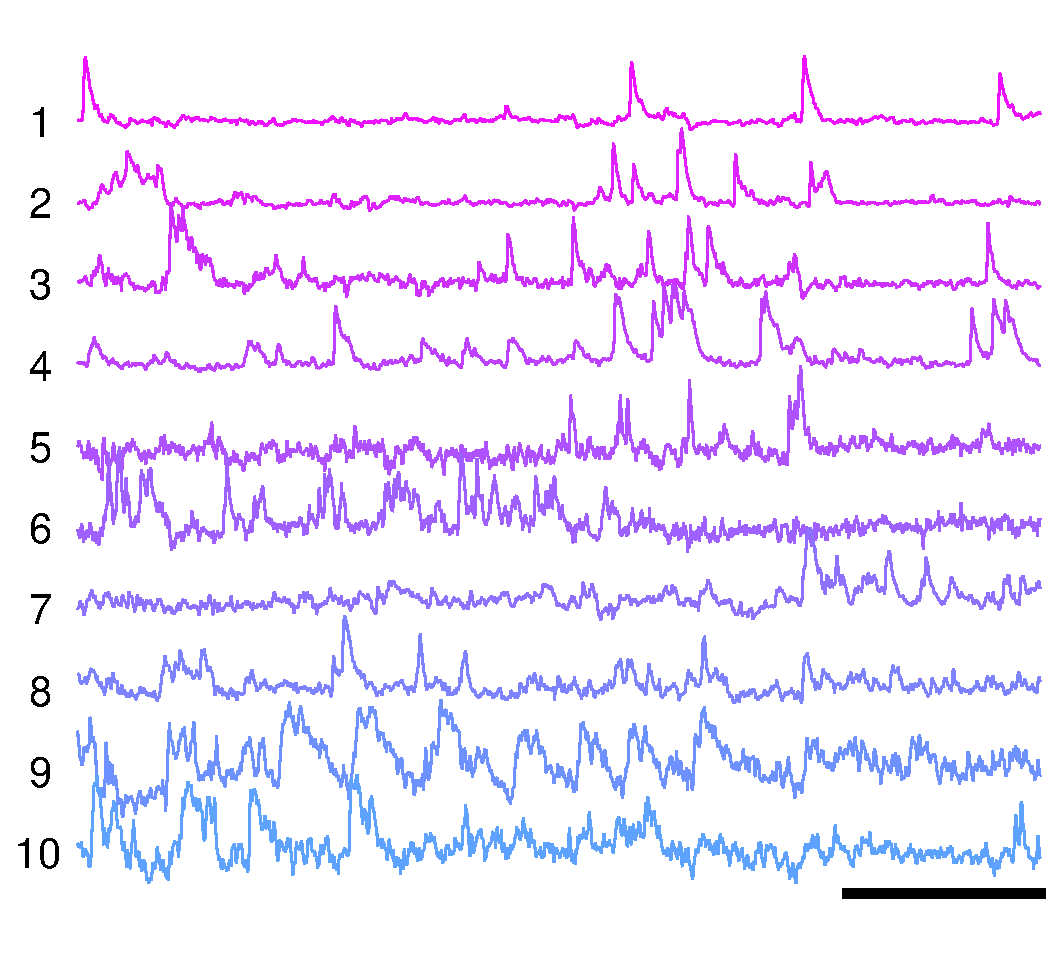
\includegraphics[height=1.65in]{Fig_PFC_subfigs/matched_temporal_cnmfe.pdf}}

\put(2.7, -5.08){\scriptsize CNMF-E traces}
\put(5.1, -5.08){\scriptsize PCA/ICA traces}

% explained variance 
\put(2.28, -3.00){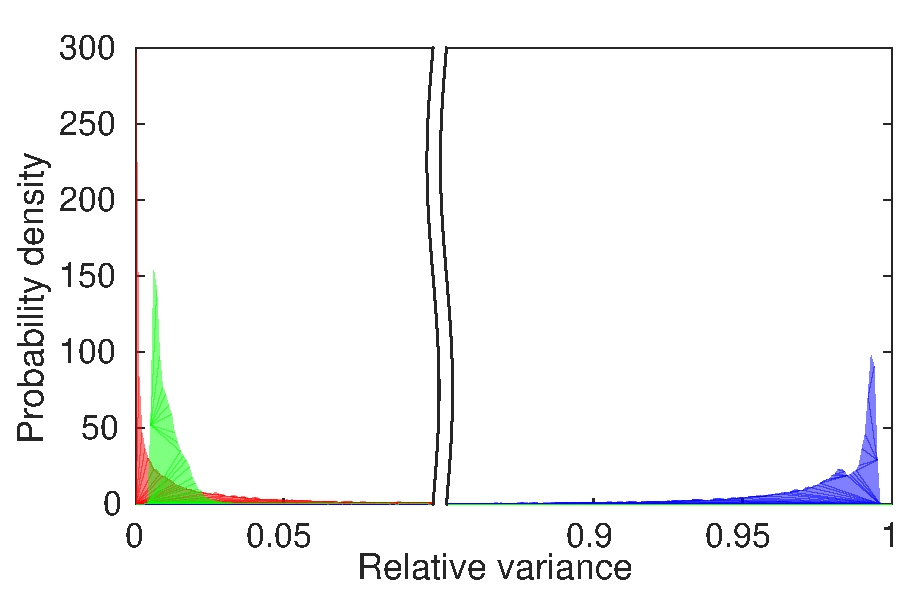
\includegraphics[height=1.5in]{Fig_PFC_subfigs/variance_explained.pdf}}
\put(2.26, -1.59){\large\textbf{C}}
\put(3.15, -1.53){\scriptsize Explained Variance}

\end{picture}
\end{document}
